\section{Resultados}

Hablar de resultados cuantitativos (tablas con las métricas en distintas pruebas) y cualitativos (imágenes resultado de cada una de las pruebas - escaladas si es necesario - con el ground truth y con la imagen real de referencia). Mencionar que para que se vean mejor las imágenes los valores se han hecho relativos para así ocupar toda la escala de grises.

%% http://www.peteryu.ca/tutorials/publishing/latex_captions_old
%% https://tex.stackexchange.com/questions/162824/vertical-spacing-between-subfloat
%% https://tex.stackexchange.com/questions/395515/how-to-scale-and-align-figures-and-tables-in-latex-in-a-3x2-grid-like-manner
\captionsetup[subfigure]{labelformat=empty}
    \begin{figure}[!ht]
\centering
    \subfloat{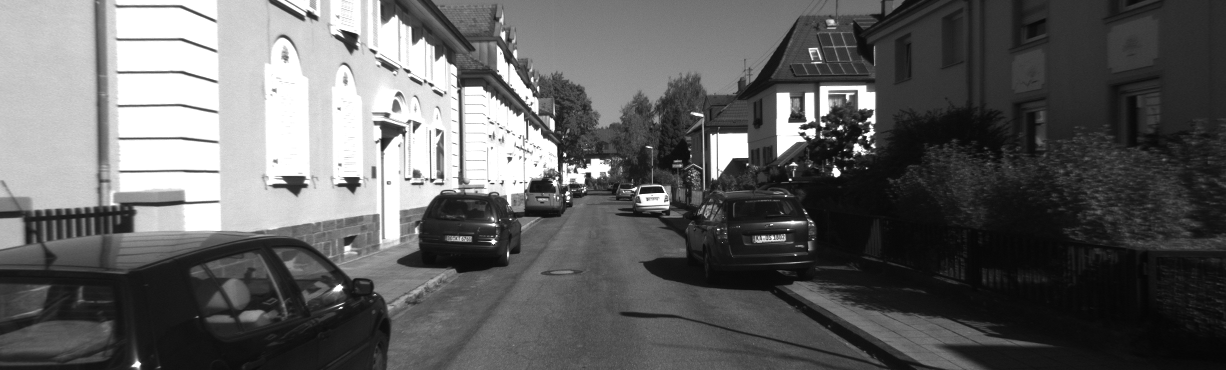
\includegraphics[width=0.33\linewidth]{imagenes/67_img0.png}}
\hfil
    \subfloat{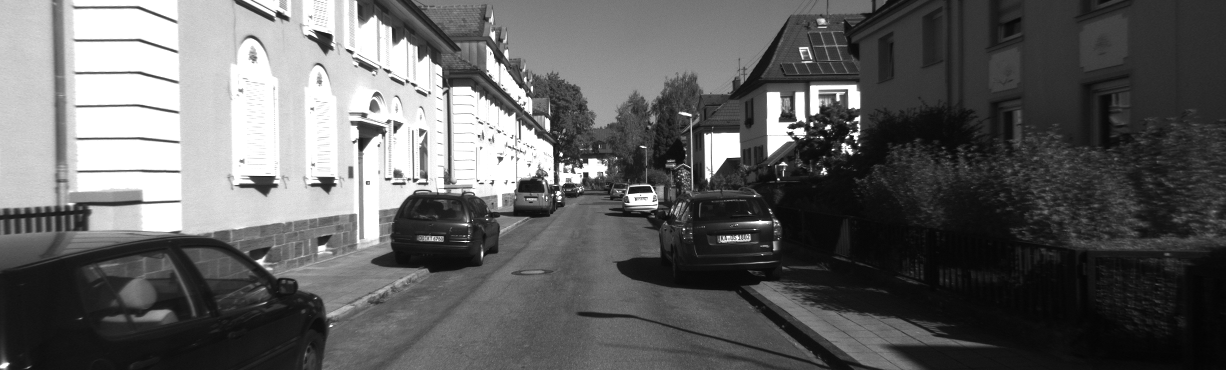
\includegraphics[width=0.33\linewidth]{imagenes/67_img1.png}}
\hfil
    \subfloat{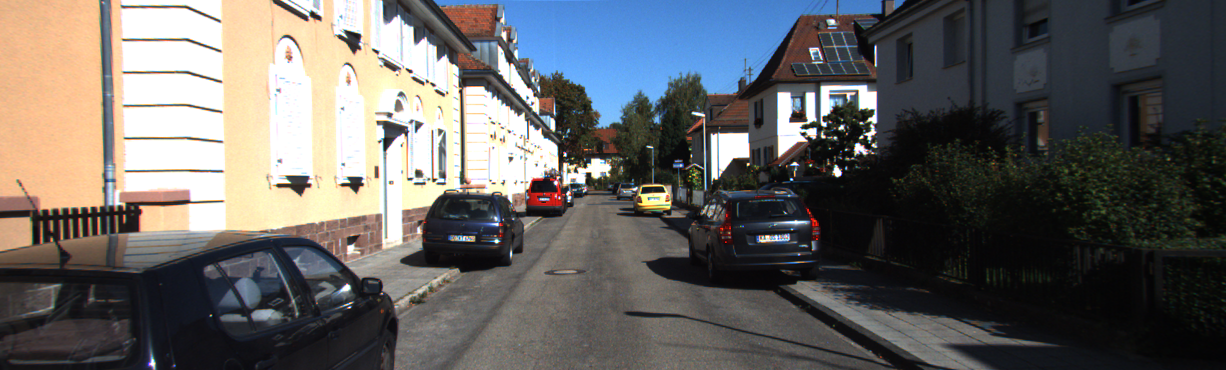
\includegraphics[width=0.33\linewidth]{imagenes/67_img2.png}}\\[-2ex]

    \subfloat{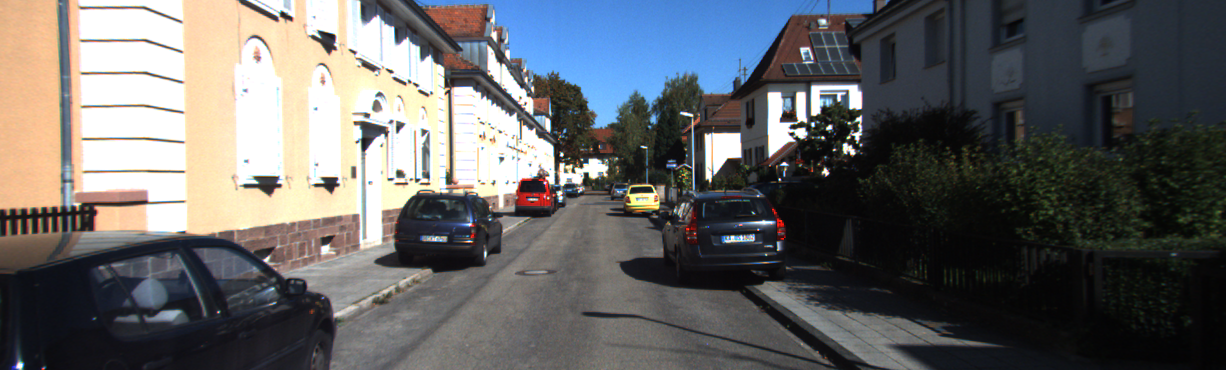
\includegraphics[width=0.33\linewidth]{imagenes/67_img3.png}}
\hfil
    \subfloat{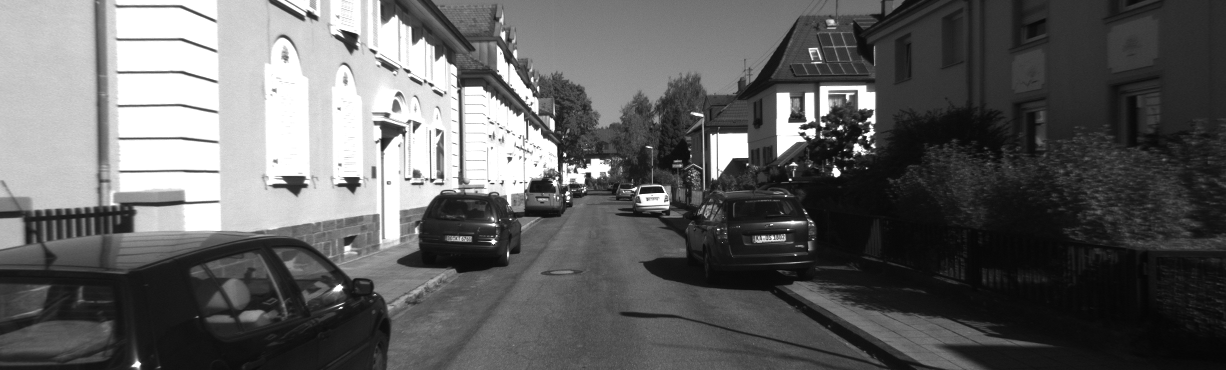
\includegraphics[width=0.33\linewidth]{imagenes/67_img0.png}}
\hfil
    \subfloat{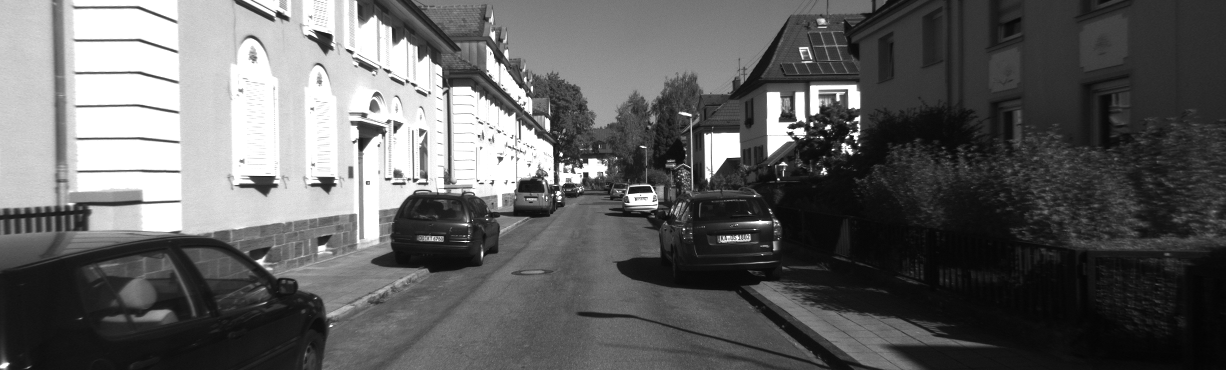
\includegraphics[width=0.33\linewidth]{imagenes/67_img1.png}}\\[-2ex]
    
    \subfloat{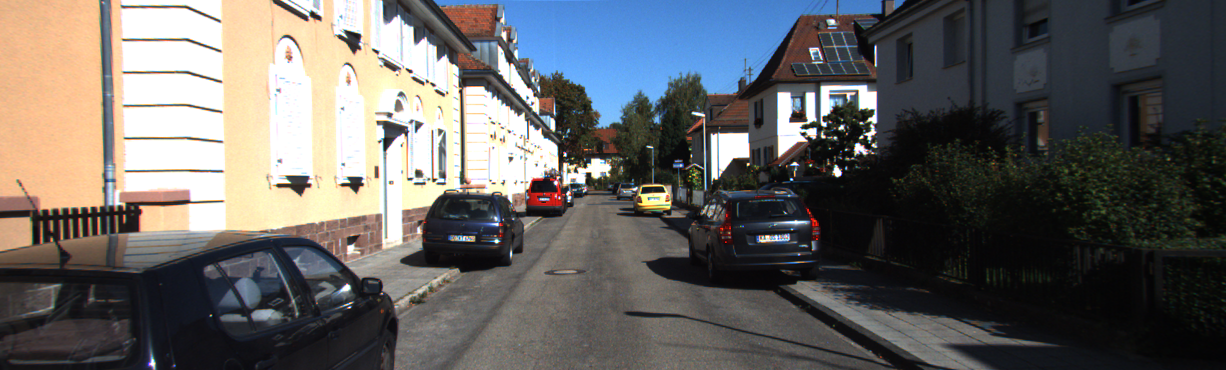
\includegraphics[width=0.33\linewidth]{imagenes/67_img2.png}}
\hfil
    \subfloat{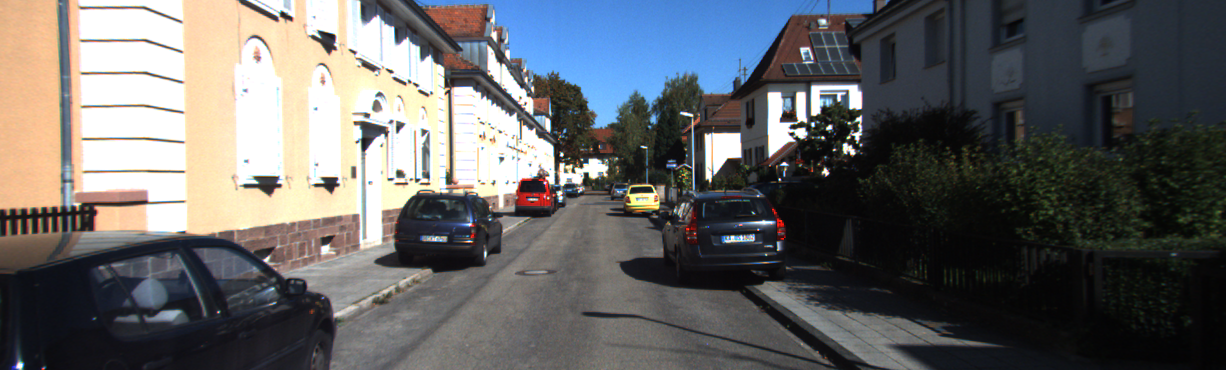
\includegraphics[width=0.33\linewidth]{imagenes/67_img3.png}}
\hfil
    \subfloat{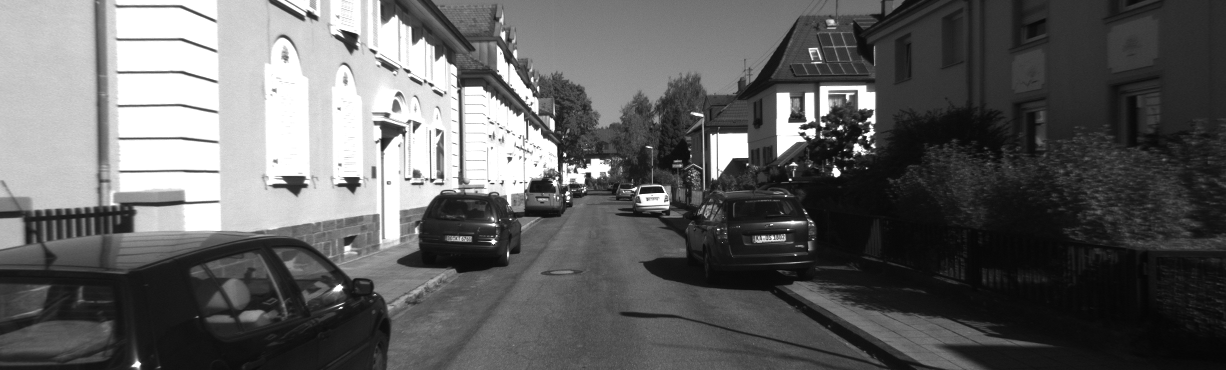
\includegraphics[width=0.33\linewidth]{imagenes/67_img0.png}}\\[-2ex]
    
    \subfloat{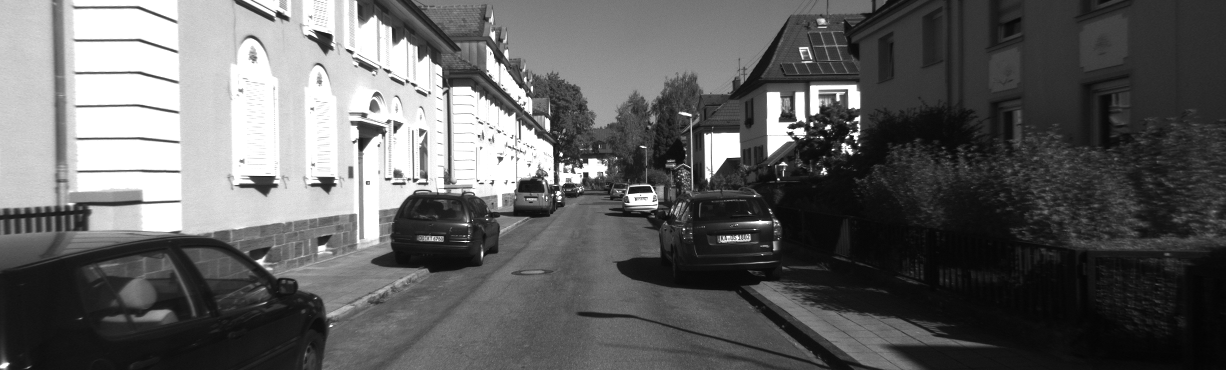
\includegraphics[width=0.33\linewidth]{imagenes/67_img1.png}}
\hfil
    \subfloat{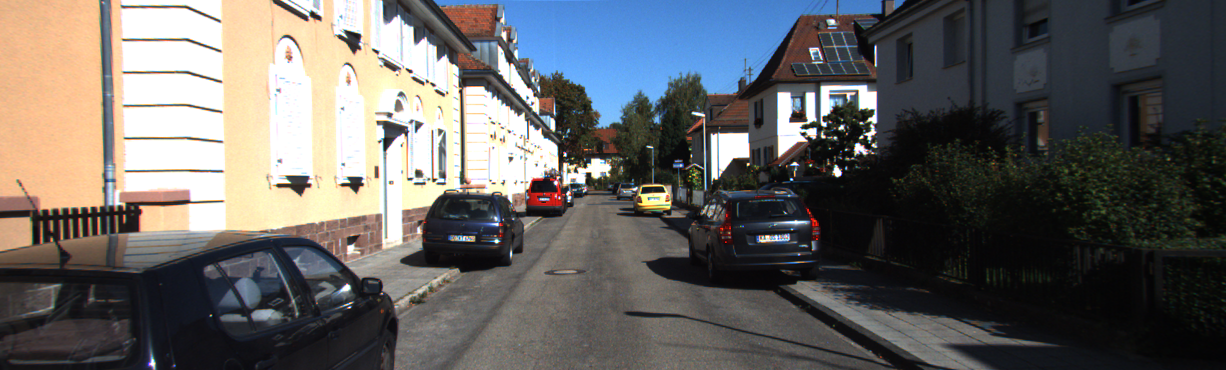
\includegraphics[width=0.33\linewidth]{imagenes/67_img2.png}}
\hfil
    \subfloat{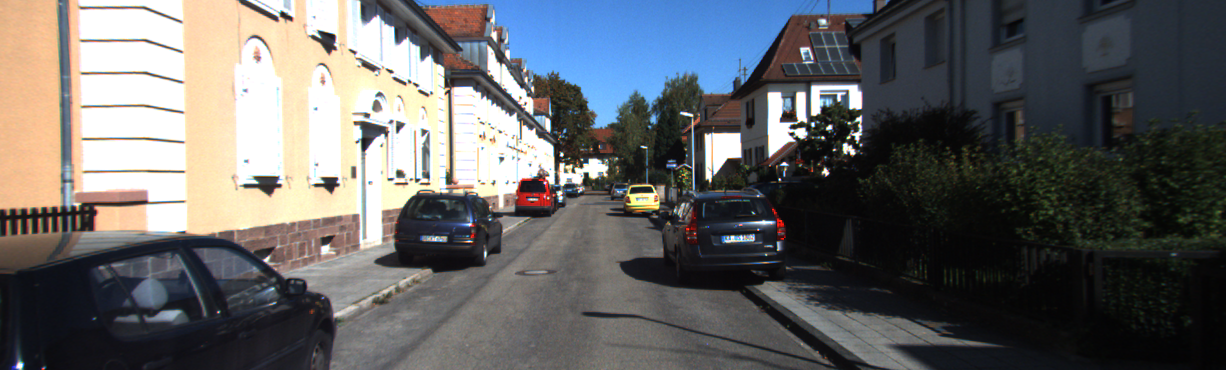
\includegraphics[width=0.33\linewidth]{imagenes/67_img3.png}}\\[-2ex]
    
    \subfloat{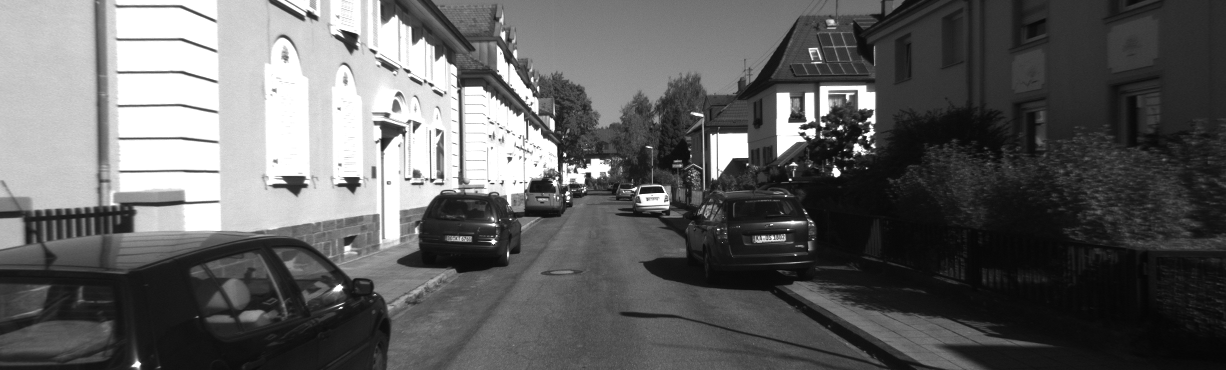
\includegraphics[width=0.33\linewidth]{imagenes/67_img0.png}}
\hfil
    \subfloat{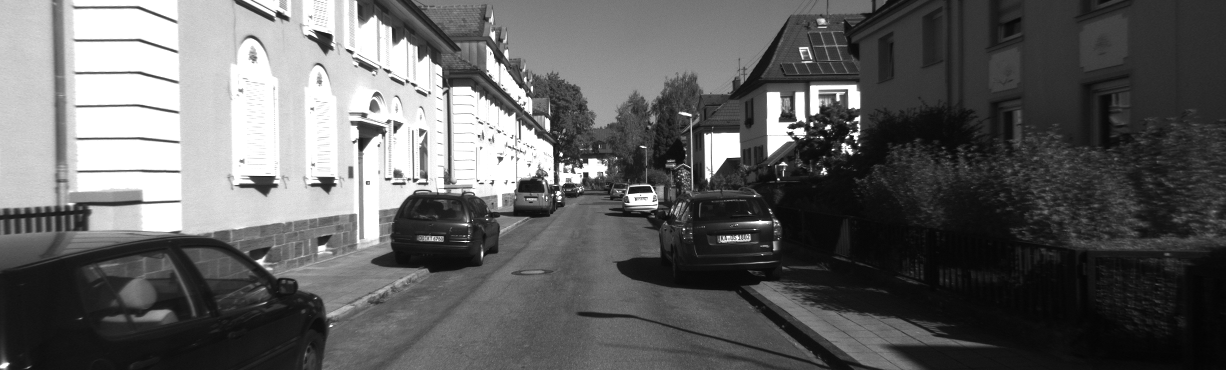
\includegraphics[width=0.33\linewidth]{imagenes/67_img1.png}}
\hfil
    \subfloat{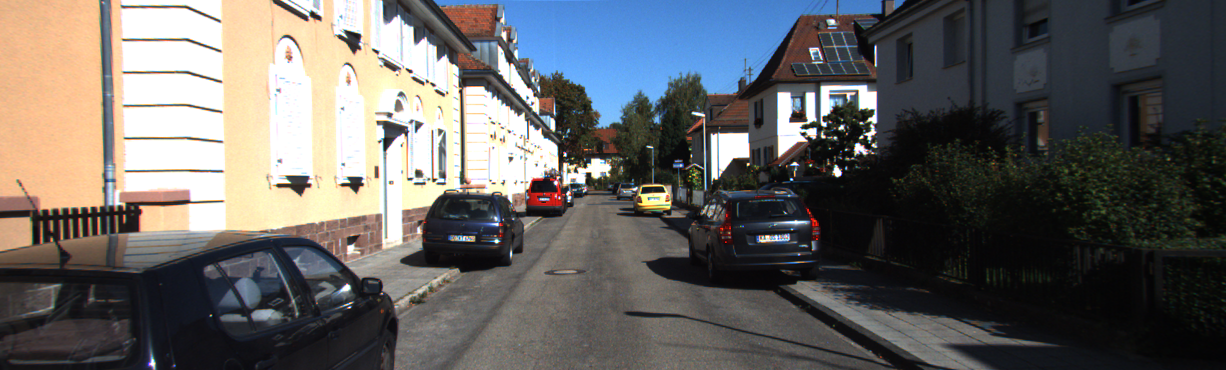
\includegraphics[width=0.33\linewidth]{imagenes/67_img2.png}}\\[-2ex]

    \subfloat{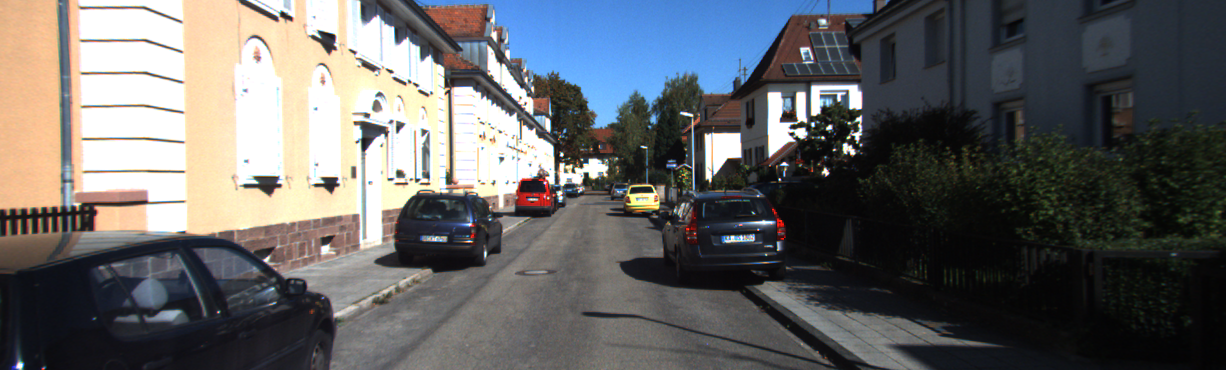
\includegraphics[width=0.33\linewidth]{imagenes/67_img3.png}}
\hfil
    \subfloat{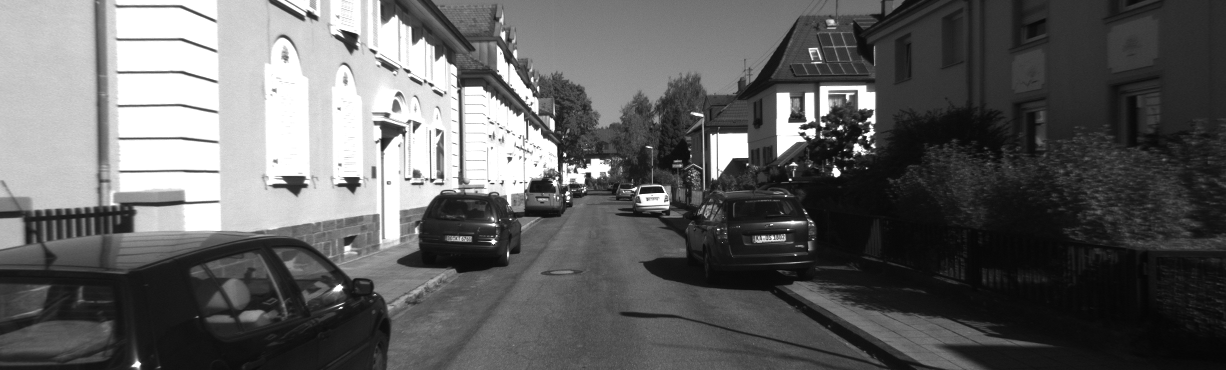
\includegraphics[width=0.33\linewidth]{imagenes/67_img0.png}}
\hfil
    \subfloat{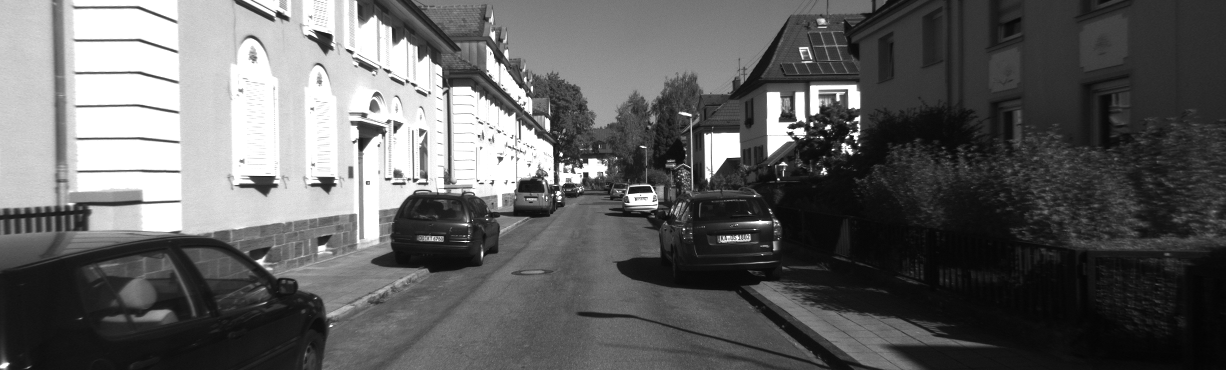
\includegraphics[width=0.33\linewidth]{imagenes/67_img1.png}}\\[-2ex]
    
    \subfloat[Entrada]{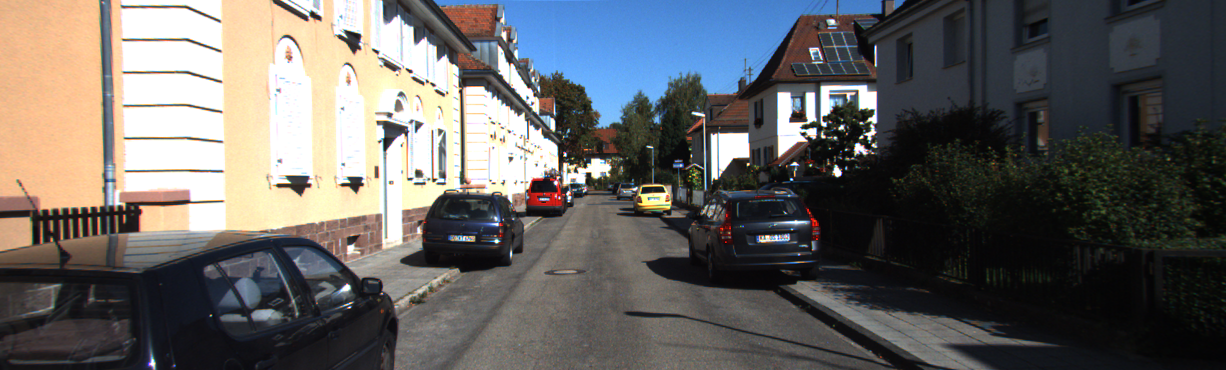
\includegraphics[width=0.33\linewidth]{imagenes/67_img2.png}}
\hfil
    \subfloat[Salida DPT modificado]{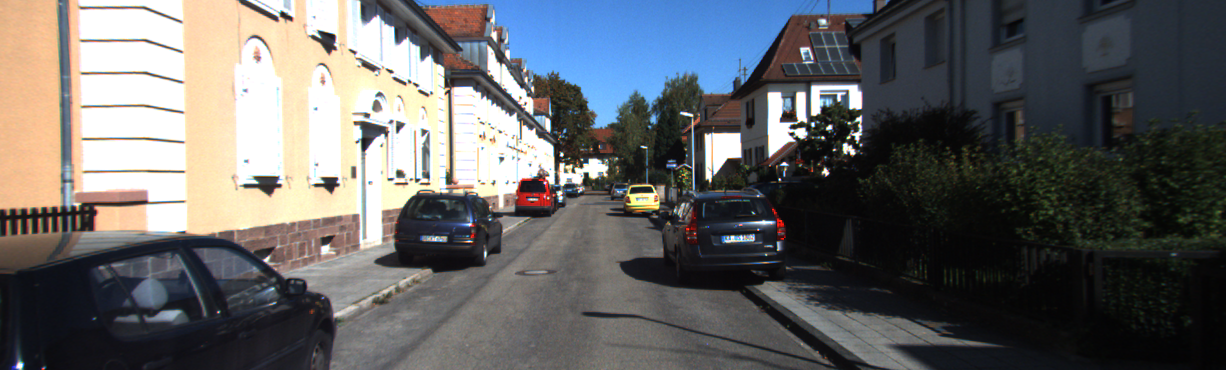
\includegraphics[width=0.33\linewidth]{imagenes/67_img3.png}}
\hfil
    \subfloat[Salida DPT sin modificar]{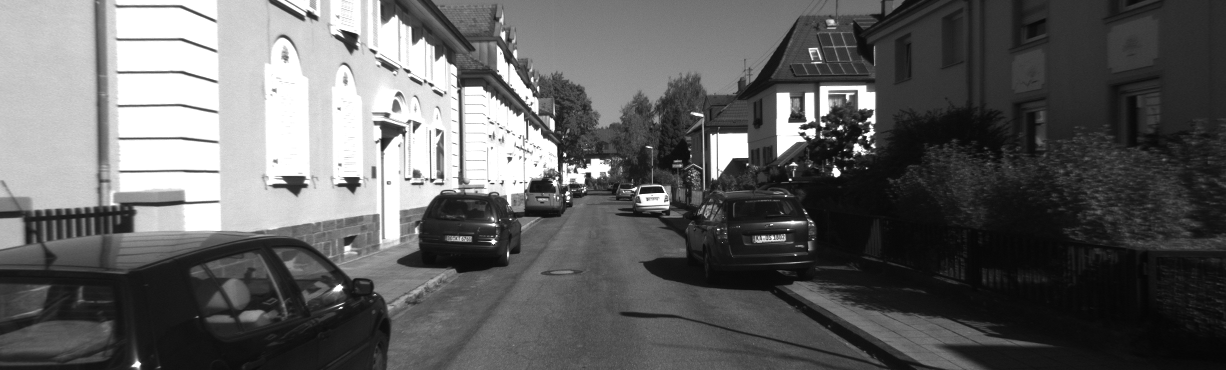
\includegraphics[width=0.33\linewidth]{imagenes/67_img0.png}}
    
\caption{Comparación cualitativa de resultados en el conjunto de evaluación entre el modelo DPT original y el modelo DPT con las modificaciones desarrolladas en este trabajo. Para facilitar su visualización, el rango de las profundidades predichas se ha ajustado a toda la escala de grises.}
    \label{fig:comparacion-cualitativa}
    \end{figure}
\captionsetup[subfigure]{labelformat=parens}

\clearpage

% Este ha sido principalmente un trabajo de revisión bibliográfica, cuyo objetivo era construir una base de conocimiento sobre la estimación de profundidades en imágenes monoculares con un cierto enfoque en las técnicas (tanto generales como específicas) capaces de acelerar dichos modelos. Por lo tanto, los resultados se presentan resumidos en el capítulo \ref{marco_teorico_estado_arte} en forma de marco teórico y estudio del estado del arte. Además de este estudio, se incluyen también en el capítulo \ref{resultados} los resultados de las pruebas de velocidad de inferencia que se han realizado en algunos de los modelos. Estas pruebas, tienen como objetivo comprobar la capacidad de modelos concretos para inferir resultados de forma online en diferente \textit{hardware}.